\chapter{हर पैमाने पर जैव विविधता}\label{ch:g10:biodiversity-scales}

किसी लॉन पर डोरी का एक मीटर का वर्ग रखिए और गिनिए कि उसके भीतर क्या-क्या
उगा है: घास तो है ही, पर तिपतिया घास, गुलबहार, एक कुकरौंधा, लुहुरिया,
मॉस भी, और लेंस से देखें तो दर्जन भर कीट और एक घोंघा भी। वही वर्ग पार्किंग
के डामर पर रख दीजिए: कुछ नहीं, या किसी दरार में एक खरपतवार। अब उसे किसी
ऐसे पुराने घास के मैदान में रखिए जिस पर कभी हल न चला हो: पौधों की चालीस
\omterm{def:g10:biodiversity-scales:species}{जातियाँ}, और कीट तो गिनती से बाहर। वह वर्ग जो नापता है उसका नाम
\emph{\omterm{def:g10:biodiversity-scales:biodiversity}{जैव विविधता}} है, और यह अध्याय इसी के बारे में है कि उसे नापा कैसे
जाए, वह किन-किन पैमानों पर मौजूद है, और वह न तो जमी हुई है, न पक्की।

\section{विविधता के तीन पैमाने}

\begin{definition}[जैव विविधता]\label{def:g10:biodiversity-scales:biodiversity}
\emph{जैव विविधता}\index{जैव विविधता} सजीवों की विविधता है, जिसे तीन
पैमानों पर देखा जाता है:
\begin{itemize}
  \item \emph{पारितंत्रों}\index{पारितंत्र} की विविधता --- यानी जीवित
        समुदायों और उनके घेरे हुए परिवेशों की (एक तालाब, एक बीच का जंगल,
        एक प्रवाल भित्ति, एक घास का मैदान), जिनमें से हर एक की अपनी
        \omterm{def:g10:biodiversity-scales:species}{जातियाँ} हैं;
  \item किसी पारितंत्र के भीतर या पूरी पृथ्वी पर \omterm{def:g10:biodiversity-scales:species}{जातियों} की विविधता
        --- यानी \omterm{def:g10:biodiversity-scales:species}{जातियों} की संख्या और उनकी सापेक्ष बहुलता;
  \item किसी \omterm{def:g10:biodiversity-scales:species}{जाति} के भीतर
        \emph{आनुवंशिक विविधता}\index{आनुवंशिक विविधता} --- यानी उसके
        \omterm{def:g10:universal-dna:gene}{जीनों} के विकल्पियों की संख्या और यह भी कि वे उसके व्यक्तियों तथा
        आबादियों में किस तरह बँटे हैं।
\end{itemize}
\end{definition}

\begin{omfigure}
\begin{tikzpicture}[font=\small, >=Stealth]
  \node[draw, rounded corners, thick, fill=omMeth!8, minimum width=11.4cm, minimum height=4.9cm] (eco) at (0,0) {};
  \node[anchor=north west, font=\small\bfseries] at (eco.north west) {\ पारितंत्र: तालाब, जंगल, भित्ति, मैदान\dots};
  \node[draw, rounded corners, thick, fill=omDef!10, minimum width=8.2cm, minimum height=3.2cm] (sp) at (0.6,-0.45) {};
  \node[anchor=north west, font=\small\bfseries] at (sp.north west) {\ एक पारितंत्र की जातियाँ};
  \foreach \x/\t in {-2.6/मेंढक, -1.1/न्यूट, 0.4/व्याध-पतंग, 1.9/नरकट, 3.4/कुमुदिनी}
    \node[draw, fill=white, rounded corners=2pt, font=\scriptsize] at (\x,-0.3) {\t};
  \node[draw, rounded corners, thick, fill=omProp!12, minimum width=6.4cm, minimum height=1.2cm] (al) at (1.0,-1.35) {};
  \node[anchor=west, font=\scriptsize\bfseries] at (al.west) {\ एक जाति के युग्मविकल्पी:};
  \foreach \x/\t in {1.6/a, 2.2/b, 2.8/c, 3.4/d, 4.0/e}
    \node[draw, circle, fill=white, inner sep=1.5pt, font=\scriptsize] at (\x,-1.35) {\t};
\end{tikzpicture}

{\small \omterm{def:g10:biodiversity-scales:biodiversity}{जैव विविधता} के तीन एक-दूसरे में धँसे पैमाने। कोई तालाब खोने पर
\omterm{def:g10:biodiversity-scales:species}{जातियों} का एक समुदाय जाता है; कोई \omterm{def:g10:biodiversity-scales:species}{जाति} खोने पर उसके सारे \omterm{def:g10:universal-dna:gene}{युग्मविकल्पी};
और \omterm{def:g10:universal-dna:gene}{युग्मविकल्पी} खोने पर वह \omterm{def:g10:biodiversity-scales:species}{जाति} दरिद्र हो जाती है जो अब भी बची हुई है।}
\end{omfigure}

\begin{definition}[जाति]\label{def:g10:biodiversity-scales:species}
\emph{जाति}\index{जाति} सजीवों का वह समूह है जो एक-दूसरे से मिलते-जुलते
हैं, आपस में प्रजनन कर सकते हैं, और उपजाऊ संतान देते हैं; जो दो आबादियाँ
आपस में प्रजनन न कर सकें, या जिनके संकर बंध्य हों, वे अलग-अलग जातियाँ
हैं। व्यवहार में --- जीवाश्मों के लिए, जीवाणुओं के लिए, और उन जीवों के
लिए जिन्हें कभी प्रजनन करते देखा नहीं गया --- जातियाँ उनके साझा
अभिलक्षणों से पहचानी जाती हैं, और
\cref{ch:g12:selection-drift-speciation} दिखाएगा कि यह सरहद हमेशा साफ़
नहीं होती।
\end{definition}

\begin{example}[घोड़ा, गधा, ख़च्चर]\label{ex:g10:biodiversity-scales:mule}
घोड़ा और गधा एक-दूसरे से मिलते-जुलते हैं और आपस में प्रजनन कर सकते हैं:
उनकी संतान ख़च्चर है। पर ख़च्चर बंध्य है, इसलिए घोड़ा और गधा दो
\omterm{def:g10:biodiversity-scales:species}{जातियाँ} हैं। पूडल और वुल्फ़हाउंड देखने में बिलकुल अलग हैं, आसानी से
प्रजनन करते हैं और उपजाऊ पिल्ले देते हैं: यानी एक ही \omterm{def:g10:biodiversity-scales:species}{जाति}, कुत्ता ---
जो अपने पूर्वज भेड़िये के साथ भी प्रजनन कर सकता है।
\end{example}

\section{जातियों की विविधता}

\begin{proposition}[जातियाँ गिनना]\label{prop:g10:biodiversity-scales:count}
लगभग बीस लाख \omterm{def:g10:biodiversity-scales:species}{जातियों} का वर्णन और नामकरण हो चुका है। इनमें अधिकांश कीट
हैं (दस लाख से ऊपर), उनके बाद पौधे (क़रीब 300\,000), कवक, अष्टपादी,
मृदुकवची; और कशेरुकी, यानी वह समूह जिसे हम सबसे अच्छा जानते हैं, लगभग
70\,000 हैं, जिनमें 6\,400 स्तनधारी। जिन \omterm{def:g10:biodiversity-scales:species}{जातियों} का वर्णन अब तक नहीं
हुआ उनकी संख्या, नई \omterm{def:g10:biodiversity-scales:species}{जातियाँ} मिलने की दर से आँकी जाए तो, कई लाख और है
--- शायद कुल मिलाकर अस्सी लाख से एक करोड़ तक सुकेंद्रकी \omterm{def:g10:biodiversity-scales:species}{जातियाँ}, और
उनके ऊपर जीवाणुओं की एक विशाल तथा बड़े हिस्से में अनगिनी विविधता।
\end{proposition}
\admitted

\begin{omfigure}
\begin{tikzpicture}
\begin{axis}[
  xbar, bar width=7pt,
  width=0.8\linewidth, height=6.4cm,
  axis x line=bottom, axis y line=left,
  xmin=0, xmax=1200,
  xlabel={वर्णित जातियाँ (हज़ारों में)},
  xlabel style={font=\small, at={(axis description cs:0.5,-0.1)}, anchor=north},
  symbolic y coords={स्तनधारी, पक्षी, मछलियाँ, मृदुकवची, अष्टपादी, कवक, पौधे, कीट},
  ytick=data, tick label style={font=\small},
  enlarge y limits=0.1,
  nodes near coords, nodes near coords style={font=\scriptsize, anchor=west},
  xtick={0,200,400,600,800,1000,1200},
]
\addplot[fill=omDef!55, draw=omDef] coordinates
  {(6.4,स्तनधारी) (11,पक्षी) (34,मछलियाँ) (85,मृदुकवची) (100,अष्टपादी)
   (150,कवक) (300,पौधे) (1000,कीट)};
\end{axis}
\end{tikzpicture}

{\small कुछ बड़े समूहों में वर्णित \omterm{def:g10:biodiversity-scales:species}{जातियाँ}, हज़ारों में। जिन समूहों को
हम सबसे अच्छा जानते हैं वही सबसे छोटे हैं; अकेले कीट सारे कशेरुकियों से
पंद्रह गुना अधिक हैं।}
\end{omfigure}

\begin{method}[किसी स्थल की विविधता नापना]\label{met:g10:biodiversity-scales:sampling}
किसी स्थल को पूरा कभी नहीं गिना जाता; उसका \emph{नमूना} लिया जाता है।
\begin{enumerate}
  \item जीवों के अनुरूप नमूना-इकाई चुनिए: घास के मैदान के पौधों के लिए
        \qty{1}{m^2} का वर्ग-खंड, कीटों के लिए जाल का एक फेरा, केंचुओं के
        लिए मिट्टी की एक छलनी, पक्षियों के लिए एक तय लंबाई की पथ-रेखा।
  \item इकाइयाँ यादृच्छिक रूप से या नियमित अंतराल पर रखिए, और इतनी रखिए
        कि एक और जोड़ने पर कुल में कम ही फ़र्क़ पड़े।
  \item हर इकाई में पहचानिए और गिनिए। नमूने का वर्णन दो संख्याएँ करती
        हैं: \emph{जाति-समृद्धि}, यानी मिली हुई \omterm{def:g10:biodiversity-scales:species}{जातियों} की संख्या,
        और हर एक की \emph{सापेक्ष बहुलता} --- जिस स्थल पर एक ही \omterm{def:g10:biodiversity-scales:species}{जाति}
        95\% व्यक्ति बनाती हो वह उस स्थल से कम विविध है जहाँ दस
        \omterm{def:g10:biodiversity-scales:species}{जातियाँ} उन्हें बराबर-बराबर बाँटती हों, चाहे समृद्धि बराबर ही
        क्यों न हो।
  \item स्थलों की तुलना केवल एक ही विधि, एक ही मेहनत और एक ही ऋतु में
        कीजिए।
\end{enumerate}
\end{method}

\begin{example}[दो लॉन]\label{ex:g10:biodiversity-scales:lawns}
किसी स्कूल के कटे हुए लॉन पर दस वर्ग-खंड: पौधों की 6 \omterm{def:g10:biodiversity-scales:species}{जातियाँ}, जिनमें
घास 90\% ढँकती है। उसी के बग़ल की बिना कटी पट्टी पर दस वर्ग-खंड: 23
\omterm{def:g10:biodiversity-scales:species}{जातियाँ}, और कोई भी 30\% से ऊपर नहीं। वह पट्टी अधिक समृद्ध और अधिक
संतुलित है; और फ़र्क़ मिट्टी या जलवायु का नहीं, जो दोनों जगह एक ही है,
बल्कि कटाई का है, जो हर उस पौधे को हटा देती है जो ज़मीन से सटकर फूल न दे
सके।
\end{example}

\begin{omfigure}
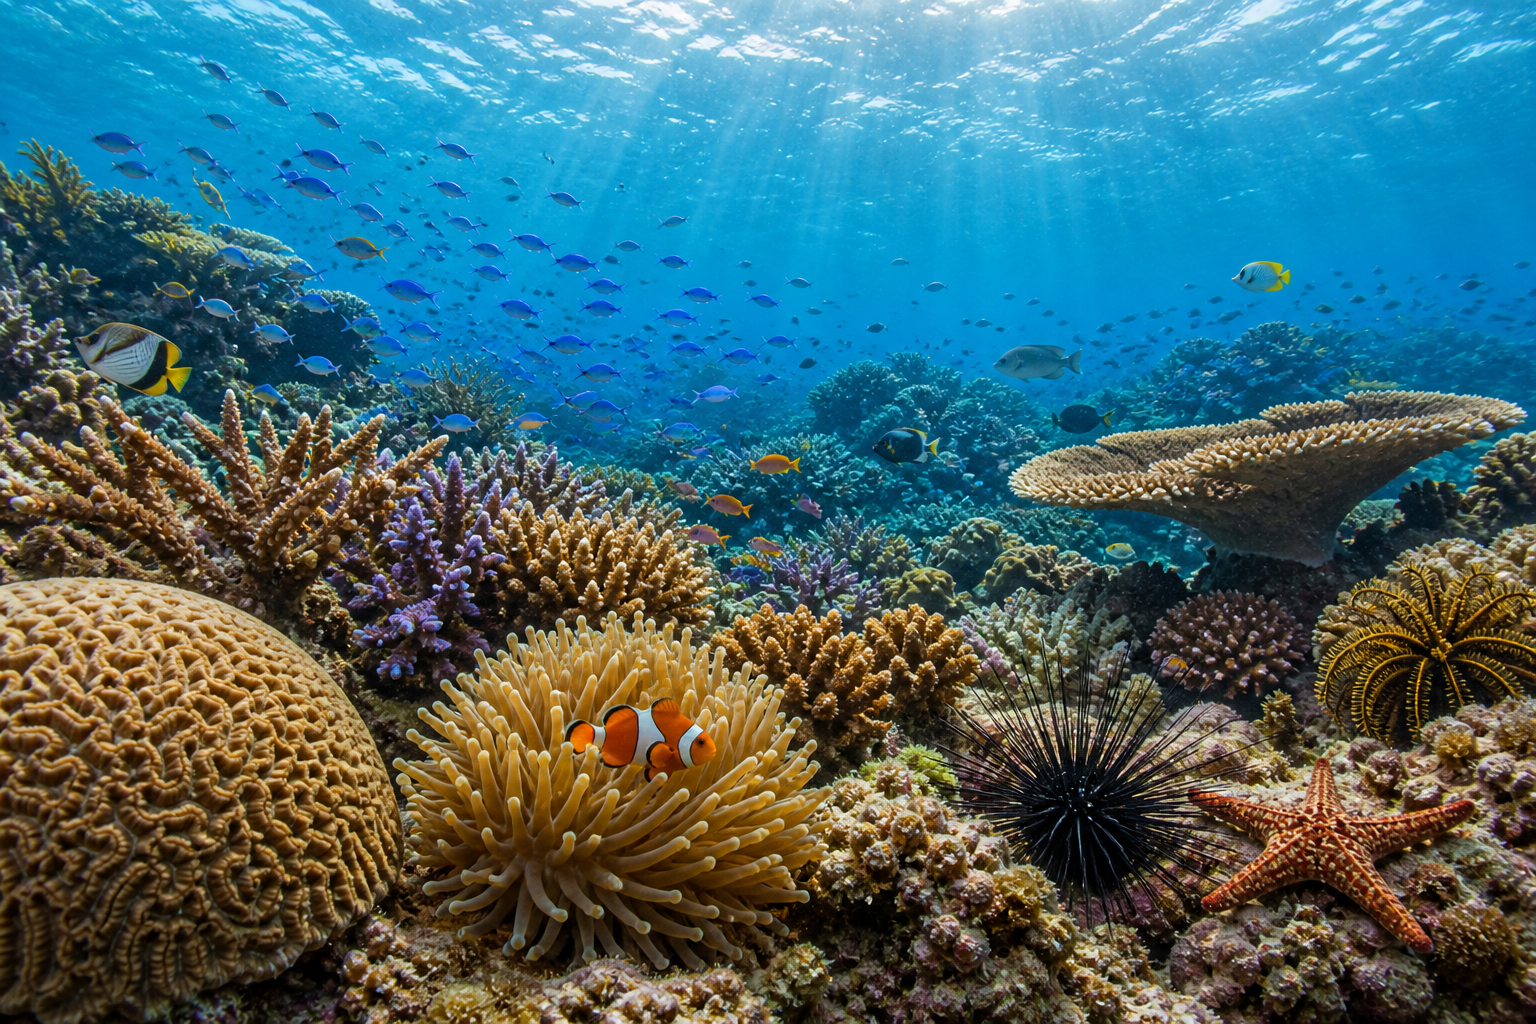
\includegraphics[width=0.66\linewidth]{images/book2/ai/g10-biodiv-coral-reef.png}

{\small एक प्रवाल भित्ति: कुछ ही वर्ग मीटर में दर्जनों \omterm{def:g10:biodiversity-scales:species}{जातियों} के
प्रवाल, मछलियाँ, मृदुकवची, शूलचर्मी और समुद्री एनीमोन। भित्तियाँ समुद्र
तल के दसवें हिस्से प्रतिशत पर सारी समुद्री \omterm{def:g10:biodiversity-scales:species}{जातियों} का चौथाई थामे हैं।}
\end{omfigure}

\section{किसी जाति के भीतर आनुवंशिक विविधता}

\begin{proposition}[किसी जाति के व्यक्ति एक जैसे नहीं होते]\label{prop:g10:biodiversity-scales:genetic}
किसी \omterm{def:g10:biodiversity-scales:species}{जाति} के भीतर अधिकांश \omterm{def:g10:universal-dna:gene}{जीन} कई विकल्पियों में मौजूद रहते हैं, और
व्यक्ति उनके अलग-अलग मेल ढोते हैं। किसी आबादी में किसी \omterm{def:g10:universal-dna:gene}{युग्मविकल्पी} की
\emph{आवृत्ति} --- यानी उस \omterm{def:g10:universal-dna:gene}{जीन} की सारी प्रतियों में से वह अंश जो यही
\omterm{def:g10:universal-dna:gene}{युग्मविकल्पी} हो --- एक आबादी से दूसरी में बदलती है। \omterm{def:g10:biodiversity-scales:biodiversity}{आनुवंशिक विविधता} ही किसी
\omterm{def:g10:biodiversity-scales:species}{जाति} को बदलते पर्यावरण का जवाब देने देती है: जिस आबादी में हर व्यक्ति
एक जैसा हो, उसके पास चुनने को कुछ बचता ही नहीं।
\end{proposition}
\admitted

\begin{example}[दुनिया भर में रक्त-समूह के युग्मविकल्पी]\label{ex:g10:biodiversity-scales:abo}
ABO रक्त-समूहों के \omterm{def:g10:universal-dna:gene}{जीन} के तीन आम \omterm{def:g10:universal-dna:gene}{युग्मविकल्पी} हैं: A, B और O. पश्चिमी यूरोप में
उनकी आवृत्तियाँ लगभग 0.27, 0.07 और 0.66 हैं; पूर्वी एशिया में लगभग 0.20,
0.20 और 0.60; और दक्षिण अमेरिका की कुछ मूल आबादियों में अकेला O \omterm{def:g10:universal-dna:gene}{युग्मविकल्पी}
0.98 तक पहुँच जाता है। वही \omterm{def:g10:biodiversity-scales:species}{जाति}, वही \omterm{def:g10:universal-dna:gene}{जीन}, पर उसके विकल्पियों का बँटवारा
अलग: मनुष्यों की \omterm{def:g10:biodiversity-scales:biodiversity}{आनुवंशिक विविधता} असली है, और वह आबादियों को बाँटने के
बजाय उन सब में फैली हुई है --- \omterm{def:g10:biodiversity-scales:species}{जाति} की अधिकांश विविधता किसी भी एक
आबादी के भीतर ही मिल जाती है।
\end{example}

\begin{omfigure}
\begin{tikzpicture}
\begin{axis}[
  ybar, bar width=9pt,
  width=0.8\linewidth, height=5.2cm,
  axis x line=bottom, axis y line=left,
  ymin=0, ymax=1.1, ylabel={युग्मविकल्पी की आवृत्ति}, ylabel style={font=\small},
  symbolic x coords={पश्चिमी यूरोप, पूर्वी एशिया, एंडीज़},
  xtick=data, tick label style={font=\small},
  enlarge x limits=0.25,
  legend style={at={(0.5,-0.2)}, anchor=north, legend columns=3,
                font=\small, draw=none},
  ytick={0,0.2,0.4,0.6,0.8,1.0},
]
\addplot[fill=omThm!50, draw=omThm] coordinates {(पश्चिमी यूरोप,0.27) (पूर्वी एशिया,0.20) (एंडीज़,0.01)};
\addplot[fill=omProp!50, draw=omProp] coordinates {(पश्चिमी यूरोप,0.07) (पूर्वी एशिया,0.20) (एंडीज़,0.01)};
\addplot[fill=omDef!50, draw=omDef] coordinates {(पश्चिमी यूरोप,0.66) (पूर्वी एशिया,0.60) (एंडीज़,0.98)};
\legend{युग्मविकल्पी A, युग्मविकल्पी B, युग्मविकल्पी O}
\end{axis}
\end{tikzpicture}

{\small मनुष्य की तीन आबादियों में ABO के तीनों विकल्पियों की अनुमानित
आवृत्तियाँ। किसी आबादी की तीनों आवृत्तियों का योग 1 होता है।}
\end{omfigure}

\begin{example}[लगभग शून्य विविधता वाली एक जाति]\label{ex:g10:biodiversity-scales:cheetah}
चीते आनुवंशिक रूप से इतने एक जैसे हैं कि आपस में असंबंधित जानवरों के बीच
त्वचा प्रत्यारोपण भी ऐसे स्वीकार हो जाते हैं जैसे जुड़वाँ के बीच हों:
यह \omterm{def:g10:biodiversity-scales:species}{जाति} क़रीब दस हज़ार साल पहले बहुत थोड़े व्यक्तियों की एक तंग गली से
गुज़री थी और उसने अपने \omterm{def:g10:universal-dna:gene}{युग्मविकल्पी} कभी वापस नहीं पाए। कोई नया रोग या जलवायु
आए, हर चीता उसका सामना उसी एक साज़-सामान से करता है; \omterm{def:g10:biodiversity-scales:species}{जाति} बची रहती है,
पर उसके पास बचाकर रखा कुछ नहीं।
\end{example}

\section{जैव विविधता बदलती है: अतीत में, आज}

\begin{proposition}[जैव विविधता एक अवस्था है, कोई स्थिरांक नहीं]\label{prop:g10:biodiversity-scales:changes}
किसी दिए हुए समय पर जीवित \omterm{def:g10:biodiversity-scales:species}{जातियों} का समुच्चय किसी इतिहास का एक पड़ाव
है। जीवाश्मों का लेखा दिखाता है कि \omterm{def:g10:biodiversity-scales:species}{जातियाँ} उभरती हैं, औसतन कुछ लाख से
कुछ करोड़ साल तक टिकती हैं, और लुप्त हो जाती हैं; पिछले 54 करोड़ साल में
जीवन की कुल विविधता बढ़ी है, पर पाँच
\emph{सामूहिक विलुप्तियों}\index{सामूहिक विलुप्ति} ने उसे तोड़ा भी है,
जिनमें भूवैज्ञानिक दृष्टि से थोड़े ही समय में तीन-चौथाई से अधिक
\omterm{def:g10:biodiversity-scales:species}{जातियाँ} ग़ायब हो गईं। सबसे हालिया विलुप्ति, 6.6 करोड़ साल पहले, बिना
पक्षी वाले डायनासोरों का अंत कर गई और स्तनधारियों के फैलाव का रास्ता खोल
गई।
\end{proposition}
\begin{proof}[साक्ष्य]
तिथि लगी चट्टान की परतों में जीवाश्म कुलों की गिनती, जो पूरे समुद्री लेखे
के लिए जोड़ी गई है, अगले चित्र का वक्र देती है: कुछ सौ से बढ़कर लगभग एक
हज़ार कुलों तक, और 44.5, 37, 25.2, 20.1 तथा 6.6 करोड़ साल पहले तीखी
गिरावटें। 25.2 करोड़ साल पहले की घटना सबसे बड़ी थी और उसने लगभग 95\%
समुद्री \omterm{def:g10:biodiversity-scales:species}{जातियाँ} मिटा दीं; उसके ठीक ऊपर की परतें जीवाश्मों से लगभग
ख़ाली हैं, और नए समूह उन्हें अगले कई लाख सालों में ही भर पाते हैं।
\end{proof}

\begin{omfigure}
\begin{tikzpicture}
\begin{axis}[
  width=0.9\linewidth, height=5.6cm,
  axis x line=bottom, axis y line=left,
  x dir=reverse, xmin=0, xmax=560, ymin=0, ymax=1100,
  xlabel={साल पहले, दस लाख की इकाइयों में}, ylabel={समुद्री जंतु कुल},
  xlabel style={font=\small, at={(axis description cs:0.5,-0.12)}, anchor=north},
  ylabel style={font=\small},
  tick label style={font=\small}, xtick={500,400,300,200,100,0},
  ytick={0,200,400,600,800,1000},
  clip=false,
]
\addplot[thick, omDef] coordinates
  {(540,120) (520,300) (490,420) (460,500) (447,510) (440,400)
   (420,470) (380,530) (368,540) (360,450) (330,480) (300,520)
   (260,540) (252,560) (248,300) (230,380) (210,440) (202,450)
   (196,380) (150,520) (100,650) (70,760) (66,780) (62,650)
   (40,760) (20,880) (0,1000)};
\draw[thick, omThm, ->] (axis cs:445,760) -- (axis cs:445,600);
\node[font=\scriptsize, omThm, anchor=south] at (axis cs:445,770) {1};
\draw[thick, omThm, ->] (axis cs:370,790) -- (axis cs:370,630);
\node[font=\scriptsize, omThm, anchor=south] at (axis cs:370,800) {2};
\draw[thick, omThm, ->] (axis cs:252,820) -- (axis cs:252,660);
\node[font=\scriptsize, omThm, anchor=south] at (axis cs:252,830) {3};
\draw[thick, omThm, ->] (axis cs:201,700) -- (axis cs:201,540);
\node[font=\scriptsize, omThm, anchor=south] at (axis cs:201,710) {4};
\draw[thick, omThm, ->] (axis cs:66,1030) -- (axis cs:66,870);
\node[font=\scriptsize, omThm, anchor=south] at (axis cs:66,1040) {5};
\end{axis}
\end{tikzpicture}

{\small समय के साथ समुद्री जंतुओं के कुलों की संख्या, जीवाश्मों के लेखे
से, और उस पर निशान लगी पाँचों सामूहिक विलुप्तियाँ (1: ऑर्डोविशियन का अंत;
2: उत्तर डिवोनियन; 3: पर्मियन का अंत, सबसे बड़ी; 4: ट्राइएसिक का अंत;
5: क्रिटेशियस का अंत)। विविधता कुल मिलाकर बढ़ती है, और हर ढहाव के बाद
धीमी बहाली आती है।}
\end{omfigure}

\begin{proposition}[आज का बदलाव]\label{prop:g10:biodiversity-scales:present}
अभी \omterm{def:g10:biodiversity-scales:species}{जातियाँ} जीवाश्म लेखे के औसत से सौ से हज़ार गुना अनुमानित दर से
ग़ायब हो रही हैं --- \omterm{def:g10:biodiversity-scales:biodiversity}{पारितंत्रों} के विनाश से (जंगल की कटाई, आर्द्रभूमियों
की निकासी, शहरीकरण), अति-दोहन से, बाहर से लाई गई \omterm{def:g10:biodiversity-scales:species}{जातियों} से, प्रदूषण
से और जलवायु परिवर्तन से --- और ये सब मानव-जनित हैं। 1950 के आधे
उष्णकटिबंधीय जंगल जा चुके हैं; उभयचरों की एक-तिहाई \omterm{def:g10:biodiversity-scales:species}{जातियाँ} ख़तरे में
हैं; और फ़सलों तथा पशुधन की \omterm{def:g10:biodiversity-scales:biodiversity}{आनुवंशिक विविधता} सिकुड़कर चंद क़िस्मों तक रह
गई है। \omterm{def:g10:biodiversity-scales:biodiversity}{जैव विविधता} एक संसाधन है --- भोजन, दवाएँ, परागण, मिट्टी,
\omterm{def:g10:biodiversity-scales:biodiversity}{पारितंत्रों} की स्थिरता --- और उसकी हानि मानवीय समय-पैमाने पर पलटी नहीं जा
सकती।
\end{proposition}
\admitted

\begin{example}[किसी हानि को पलटना]\label{ex:g10:biodiversity-scales:reversing}
जहाँ 1960 के दशक में हटाई गई झाड़ीदार बाड़ें दोबारा लगाई गईं, वहाँ पक्षियों
और कीटों की समृद्धि दस साल के भीतर लौट आई; और जहाँ 1995 में किसी राष्ट्रीय
उद्यान में भेड़िये दोबारा बसाए गए, वहाँ जिन हिरनों का वे शिकार करते हैं
उन्होंने नदी किनारे के विलो छीलने बंद कर दिए, विलो फिर उग आए, बीवर लौट
आए, और उनके साथ वे पक्षी तथा मछलियाँ भी जो बीवरों के तालाबों पर टिकी हैं।
किसी \omterm{def:g10:biodiversity-scales:biodiversity}{पारितंत्र} को बचाना या बहाल करना तीनों पैमानों पर एक साथ विविधता लौटा
देता है; चिड़ियाघर में जीवित रखी गई कोई \omterm{def:g10:biodiversity-scales:species}{जाति} उनमें से केवल एक बचाती है।
\end{example}

\section{अभ्यास}

\begin{exercise}[$\star$]\label{exo:g10:biodiversity-scales:1}
\omterm{def:g10:biodiversity-scales:biodiversity}{जैव विविधता} के तीनों पैमानों के नाम लिखिए और हर एक का एक उदाहरण दीजिए।
\end{exercise}

\begin{exercise}[$\star$]\label{exo:g10:biodiversity-scales:2}
\omterm{def:g10:biodiversity-scales:species}{जाति} की परिभाषा दीजिए। शेर और बाघ --- जो क़ैद में बंध्य संकर दे सकते
हैं --- एक \omterm{def:g10:biodiversity-scales:species}{जाति} हैं या दो?
\end{exercise}

\begin{exercise}[$\star$]\label{exo:g10:biodiversity-scales:3}
\omterm{def:g10:biodiversity-scales:species}{जातियों} वाले आलेख से बताइए कि स्तनधारी \omterm{def:g10:biodiversity-scales:species}{जातियों} से कितने गुना अधिक
कीट \omterm{def:g10:biodiversity-scales:species}{जातियों} का वर्णन हुआ है।
\end{exercise}

\begin{exercise}[$\star$]\label{exo:g10:biodiversity-scales:4}
\omterm{def:g10:universal-dna:gene}{युग्मविकल्पी} की आवृत्ति क्या है? जिस आबादी में O \omterm{def:g10:universal-dna:gene}{युग्मविकल्पी} की आवृत्ति 0.66 और A
\omterm{def:g10:universal-dna:gene}{युग्मविकल्पी} की 0.27 हो, उसमें B की आवृत्ति क्या है?
\end{exercise}

\begin{exercise}[$\star$]\label{exo:g10:biodiversity-scales:5}
जीवाश्मों का लेखा कितनी सामूहिक विलुप्तियाँ दिखाता है, और उनमें सबसे बड़ी
कौन-सी थी?
\end{exercise}

\begin{exercise}[$\star\star$]\label{exo:g10:biodiversity-scales:6}
दो घास के मैदानों में से हर एक में पौधों की 12 \omterm{def:g10:biodiversity-scales:species}{जातियाँ} हैं। पहले में
एक ही \omterm{def:g10:biodiversity-scales:species}{जाति} 80\% पौधे बनाती है; दूसरे में कोई भी \omterm{def:g10:biodiversity-scales:species}{जाति} 15\% से ऊपर
नहीं। कौन-सा अधिक विविध है, और
\cref{met:g10:biodiversity-scales:sampling} की दोनों संख्याओं में से
कौन-सी उन्हें अलग बताती है?
\end{exercise}

\begin{exercise}[$\star\star$]\label{exo:g10:biodiversity-scales:7}
एक विद्यार्थी जाल के 3 फेरों में कीट गिनता है और 8 \omterm{def:g10:biodiversity-scales:species}{जातियाँ} पाता है;
उसका सहपाठी उसी खेत में 30 फेरे लगाता है और 21 पाता है। क्या उस सहपाठी के
लिए खेत में अधिक \omterm{def:g10:biodiversity-scales:species}{जातियाँ} हैं? समझाइए कि यह फ़र्क़ नमूना लेने के बारे
में क्या दिखाता है।
\end{exercise}

\begin{exercise}[$\star\star$]\label{exo:g10:biodiversity-scales:8}
समझाइए कि चंद दर्जन व्यक्तियों तक सिमट चुकी कोई \omterm{def:g10:biodiversity-scales:species}{जाति} अपनी संख्या
दोबारा हज़ारों में पहुँच जाने के बाद भी ख़तरे में क्यों रह सकती है।
\end{exercise}

\begin{exercise}[$\star\star$]\label{exo:g10:biodiversity-scales:9}
जीवाश्म कुलों वाले चित्र में 25.2 करोड़ साल पहले की विलुप्ति से ठीक पहले
और ठीक बाद के कुलों की संख्या पढ़िए, और खोया हुआ अंश निकालिए। खोई हुई
\emph{\omterm{def:g10:biodiversity-scales:species}{जातियों}} का अंश कुलों के अंश से बड़ा क्यों है?
\end{exercise}

\begin{exercise}[$\star\star$]\label{exo:g10:biodiversity-scales:10}
\cref{ex:g10:biodiversity-scales:abo} की मदद से समझाइए कि किस अर्थ में एक
ही शहर के दो पड़ोसी आनुवंशिक रूप से लगभग उतने ही अलग होने की संभावना रखते
हैं जितने अलग-अलग महाद्वीपों के दो लोग।
\end{exercise}

\begin{exercise}[$\star\star$]\label{exo:g10:biodiversity-scales:11}
किसी तालाब को सुखाकर वहाँ पार्किंग बनाई जाती है। \omterm{def:g10:biodiversity-scales:biodiversity}{जैव विविधता} के तीनों
पैमानों में से हर एक पर एक-एक हानि गिनाइए।
\end{exercise}

\begin{exercise}[$\star\star\star$]\label{exo:g10:biodiversity-scales:12}
जीवाश्म लेखे की औसत \omterm{def:g10:biodiversity-scales:species}{जाति} कुछ लाख से कुछ करोड़ साल टिकती है; बीस लाख
ज्ञात \omterm{def:g10:biodiversity-scales:species}{जातियों} के साथ प्रति वर्ष विलुप्तियों की ``पृष्ठभूमि'' संख्या
आँकिए। यदि आज की दर उससे हज़ार गुना हो, तो प्रति वर्ष कितनी \omterm{def:g10:biodiversity-scales:species}{जातियाँ}
ग़ायब होंगी, और प्रति सदी कितनी?
\end{exercise}

\begin{exercise}[$\star\star\star$]\label{exo:g10:biodiversity-scales:13}
6.6 करोड़ साल पहले की विलुप्ति के बाद स्तनधारी चंद छोटे रूपों से फैलकर
क़रीब 2 करोड़ साल के भीतर ह्वेल, चमगादड़, हाथी और नरवानर बन गए। समझाइए
कि \omterm{def:g10:biodiversity-scales:biodiversity}{जैव विविधता} की कोई आपदा नई \omterm{def:g10:biodiversity-scales:biodiversity}{जैव विविधता} का कारण भी कैसे बन सकती है।
\end{exercise}

\begin{exercise}[$\star\star\star$]\label{exo:g10:biodiversity-scales:14}
आधुनिक गेहूँ मुट्ठी भर क़िस्मों से उतरा है; उसके जंगली नातेदार मध्य पूर्व
के पहाड़ों में उगते हैं। \omterm{def:g10:biodiversity-scales:biodiversity}{आनुवंशिक विविधता} की धारणा से समझाइए कि बीज बैंक
उन जंगली नातेदारों को क्यों सँभालकर रखते हैं, जबकि उनसे काम लायक़ कुछ
मिलता ही नहीं।
\end{exercise}

\begin{exercise}[$\star\star\star$]\label{exo:g10:biodiversity-scales:15}
``विलुप्ति प्राकृतिक है, इसलिए आज की विलुप्ति पर चिंता की कोई वजह नहीं।''
विलुप्ति की दर, बहाली में लगने वाले समय, और \omterm{def:g10:biodiversity-scales:biodiversity}{जैव विविधता} से मिलने वाले
संसाधनों की मदद से एक अनुच्छेद में इस पर चर्चा कीजिए।
\end{exercise}

\section{समस्या: बाड़ का लाभांश}

\begin{problem}[{सप्ताहांत समस्या --- दो खेतों का क्षेत्र-सर्वेक्षण, एक
बाड़ों वाला और एक बिना बाड़ का: जातियाँ गिनी गईं, बहुलताएँ तुलनाई गईं,
एक घोंघे के युग्मविकल्पी पीछा किए गए, और वह संख्या जिसके बराबर कोई बाड़ है}]
\label{pb:g10:biodiversity-scales:1}
पड़ोस के दो खेत एक ही मिट्टी पर एक ही गेहूँ उगाते हैं। खेत A ने अपनी
झाड़ीदार बाड़ें रखीं; खेत B ने उन्हें 1970 में हटा दिया। एक कक्षा जून में
दोनों का एक ही विधि से नमूना लेती है: पौधों के लिए खेत के किनारों के
साथ-साथ \qty{1}{m^2} के 20 वर्ग-खंड, कीटों के लिए जाल के 20 फेरे, और
पक्षियों के लिए 5 बिंदुओं पर 10 मिनट का सुनना।

\medskip
\noindent\textbf{भाग I --- पौधे।}
नतीजे, खेत A: 20 वर्ग-खंडों में पौधों की 31 \omterm{def:g10:biodiversity-scales:species}{जातियाँ}; खेत B: 9.
खेत B पर एक ही घास गिने गए पौधों का 84\% बनाती है; खेत A पर सबसे आम
\omterm{def:g10:biodiversity-scales:species}{जाति} 22\% बनाती है।
\begin{enumerate}
  \item हर खेत के किनारों की जाति-समृद्धि बताइए और दोनों का अनुपात
        भी।
  \item किस खेत का पादप समुदाय अधिक संतुलित है? समझाइए कि
        ``संतुलित'' शब्द ``समृद्ध'' में क्या जोड़ता है।
  \item खेत A पर 5, 10, 15 और 20 वर्ग-खंडों के बाद मिली \omterm{def:g10:biodiversity-scales:species}{जातियों} की
        संख्या 18, 25, 29 और 31 थी। क्या नमूना पर्याप्त है? कारण
        बताइए।
  \item खेत B पर यही शृंखला 6, 8, 9, 9 थी। दोनों शृंखलाओं की तुलना
        कीजिए और बताइए कि किसी ``पूरे'' नमूना-वक्र का आकार कैसा होता है।
  \item दोनों खेतों का नमूना एक ही महीने में क्यों लेना चाहिए?
\end{enumerate}

\medskip
\noindent\textbf{भाग II --- कीट और पक्षी।}
कीट: खेत A 46 \omterm{def:g10:biodiversity-scales:species}{जातियाँ}, खेत B 14. पक्षी: खेत A 17 \omterm{def:g10:biodiversity-scales:species}{जातियाँ}, खेत B
5; और खेत B पर सुने गए 60\% पक्षी एक ही \omterm{def:g10:biodiversity-scales:species}{जाति} के थे।
\begin{enumerate}[resume]
  \item दोनों खेतों के बीच कीट-समृद्धि और पक्षी-समृद्धि का अनुपात
        निकालिए। क्या तीनों समूह (पौधे, कीट, पक्षी) एक ही कहानी कहते
        हैं?
  \item बाड़ें हटाने से कीटों की विविधता के गिरने तक, और फिर पक्षियों की
        विविधता तक, कारणों की एक शृंखला सुझाइए।
  \item दोनों खेतों में प्रति हेक्टेयर गेहूँ की उपज एक ही है। तो क्या
        इसका मतलब है कि बाड़ों का फ़सल पर कोई असर नहीं? कोई एक सेवा
        सुझाइए जो बाड़ दे सकती है और जो उपज के आँकड़े में नहीं दिखती।
  \item ऐसी एक \omterm{def:g10:biodiversity-scales:species}{जाति} का नाम लीजिए जिसे कक्षा केवल खेत A पर मिलने की
        उम्मीद करेगी, और कारण भी बताइए।
  \item खेत B पर \omterm{def:g10:biodiversity-scales:biodiversity}{जैव विविधता} का कौन-सा पैमाना सबसे साफ़ तौर पर घटा है:
        \omterm{def:g10:biodiversity-scales:biodiversity}{पारितंत्र}, \omterm{def:g10:biodiversity-scales:species}{जातियाँ}, या \omterm{def:g10:universal-dna:gene}{जीन}? कारण बताइए।
\end{enumerate}

\medskip
\noindent\textbf{भाग III --- एक घोंघे के \omterm{def:g10:universal-dna:gene}{युग्मविकल्पी}।}
बग़ीचे के घोंघे में खोल के रंग का एक \omterm{def:g10:universal-dna:gene}{जीन} है जिसके दो आम \omterm{def:g10:universal-dna:gene}{युग्मविकल्पी} हैं,
पीला (y) और भूरा (b)। खेत A की बाड़ों में 400 घोंघों का नमूना लिया गया:
100 में दो y \omterm{def:g10:universal-dna:gene}{युग्मविकल्पी} हैं, 200 में एक y और एक b, और 100 में दो b। खेत B
की बची हुई एक मेड़ पर 100 घोंघे: 4 में दो y, 32 में एक-एक, 64 में दो b।
\begin{enumerate}[resume]
  \item हर नमूने में y और b की प्रतियाँ गिनिए (हर घोंघा दो प्रतियाँ ढोता
        है)। इससे हर खेत पर y की आवृत्ति निकालिए।
  \item इस \omterm{def:g10:universal-dna:gene}{जीन} पर कौन-सी आबादी आनुवंशिक रूप से अधिक विविध है? दोनों
        \omterm{def:g10:universal-dna:gene}{युग्मविकल्पी} ढोने वाले घोंघों के अनुपात की तुलना कीजिए।
  \item थ्रश घोंघों का शिकार देखकर करते हैं; खेत B की उजाड़ मेड़ पर भूरे
        खोल बेहतर छिपते हैं। सुझाइए कि खेत B की आवृत्तियाँ कैसे बनीं।
  \item यदि कोई नम, छायादार बाड़ पीले खोलों के पक्ष में हो, तो बाड़ें
        दोबारा लगाने पर और कुछ न बदलने पर खेत B के घोंघों के लिए आप क्या
        अनुमान लगाएँगे?
  \item खेत B के घोंघे कुछ सौ हैं; खेत A के दसियों हज़ार। कौन-सी आबादी
        संयोग से किसी \omterm{def:g10:universal-dna:gene}{युग्मविकल्पी} को पूरी तरह खो देने के प्रति अधिक खुली है?
        क्यों?
\end{enumerate}

\medskip
\noindent\textbf{भाग IV --- लाभांश।}
\begin{enumerate}[resume]
  \item तीनों समूहों को मिलाकर हर खेत की कुल जाति-समृद्धि निकालिए,
        फिर खेत A का कुल खेत B के कुल से भाग दीजिए।
  \item खेत A की बाड़ें उसके क्षेत्रफल का 3\% घेरती हैं। एक वाक्य में
        बताइए कि ज़मीन का कितना अंश \omterm{def:g10:biodiversity-scales:species}{जातियों} का कितना अंश थामे हुए है।
  \item खेत B पर 1995 में दोबारा लगाई गई बाड़ों का 2010 में फिर
        सर्वेक्षण हुआ: पौधे 24, कीट 35, पक्षी 12 \omterm{def:g10:biodiversity-scales:species}{जातियाँ}। हर समूह ने
        खेत A की समृद्धि का कितना अंश वापस पाया?
  \item दोबारा लगाने के बाद \omterm{def:g10:biodiversity-scales:biodiversity}{जैव विविधता} का कौन-सा पैमाना सबसे धीरे लौटता
        है, और क्यों?
  \item परिणाम लिखिए: बाड़ों ने किसी खेत की जाति-समृद्धि कितने गुना
        बढ़ाई, और \omterm{def:g10:biodiversity-scales:biodiversity}{जैव विविधता} का वह एक पैमाना कौन-सा है जिसे दोबारा लगाई
        गई बाड़ अपने बल पर वापस नहीं ला सकती।
\end{enumerate}
\end{problem}
